\section{$\Delta$Q display}
    Now that we have introduced the required concepts, we can put everything together to be plotted. In summary, a probe's displayed graph must contain:
    \begin{itemize}
        \item The observed $\Delta$Q of the sampling window, with the mean and confidence bounds calculated over the polling window of observed $\Delta$Qs.
        \item If applicable, the calculated $\Delta$Q of the sampling window from the causally linked components observed in a probe, with the mean and confidence bounds calculated over the polling window of calculated $\Delta$Qs.
        \item Its QTA (if defined).
    \end{itemize}
    This allows for the user to observe if a $\Delta$Q has deviated from normal execution, analyse its stationarity, non-linearity and observe a sampled $\Delta$Q over a polling window.

    In the screenshot below (\cref{fig:dq_displ}) we can observe the multiple elements as they are displayed in real time in the oscilloscope.
    \begin{itemize}
        \item (1, green): The mean of the polling window observed $\Delta$Qs (yellow) with the confidence bounds. Upper bound (dark green) and lower bound (light green). The observed $\Delta$Q of the sampling window (blue) can be observed going out of the confidence bounds at delay 0.00125 s. The $\Delta$Q in a sampling window is less precise than the mean and confidence bounds calculated in the polling window.
        \item (2, red): The mean of the calculated $\Delta$Qs (ochre) with the confidence bounds of the mean. Upper bound (purple) and lower bound (magenta). The calculated $\Delta$Q of the sampling window (red) is inside its confidence bounds.
        \item (3, blue): The \textbf{QTA}.
    \end{itemize}
     \begin{figure}[H]
        \begin{center}
            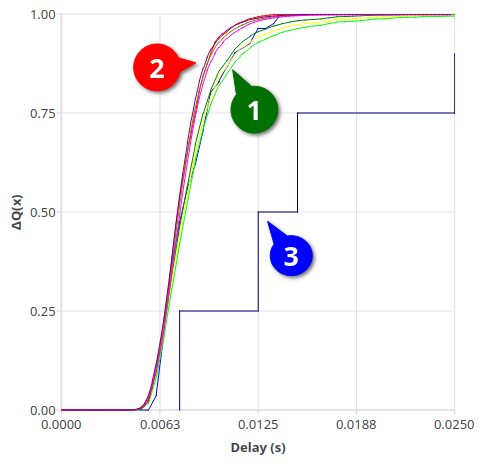
\includegraphics[scale = 0.7]{img/overload_2/fired_sampleb.png}
        \end{center}
         \caption{$\Delta$Qs, confidence bounds, means and QTA for a probe observing the causal link of multiple components.}
         \label{fig:dq_displ}
    \end{figure}
        

